\documentclass[a4paper]{article}

\usepackage[portuguese]{babel} \usepackage[utf8]{inputenc}
%\usepackage{indentfirst}
\usepackage{graphicx}
\usepackage{verbatim}
\usepackage[T1]{fontenc}
\usepackage{wrapfig}
\usepackage[tmargin=1.2in,bmargin=1in]{geometry}
\usepackage{listingsutf8}
\usepackage[utf8]{inputenc}
\usepackage{color}
\usepackage{ucs}
\usepackage{etoolbox}
\AtBeginEnvironment{tabular}{\noindent}
\setlength\parindent{0pt}

\begin{document}

\setlength{\textwidth}{16cm} \setlength{\textheight}{22cm}

\title{\Huge\textbf{Rede de Computadores}\linebreak\linebreak\linebreak\linebreak \Large\textbf{Relatório \\
    Trabalho2}\linebreak\linebreak\linebreak
\includegraphics[height=6cm,
    width=7cm]{feup.pdf}\linebreak \linebreak \Large{Mestrado Integrado em
    Engenharia Informática e Computação} \linebreak \linebreak \Large\textbf{Redes de
Computadores}\linebreak}

\author{Hugo Ari Rodrigues Drumond --- 201102900 --- hugo.drumond@fe.up.pt \\
    José Pedro Pereira Amorim --- 201206111 --- ei12190@fe.up.pt \\ João
    Ricardo Pintas Soares --- 201200740 ---
    ei12039@fe.up.pt\linebreak\linebreak\linebreak \\ \\ Faculdade de
    Engenharia da Universidade do Porto \\ Rua Roberto Frias, 4200--65 Porto,
    Portugal \linebreak\linebreak\linebreak \linebreak\linebreak\vspace{1cm}}
    \maketitle \thispagestyle{empty}

\newpage

\section{Introdução}
Este trabalho laboratorial, desenvolvido no âmbito da Unidade Curricular de
Redes de Computadores (RCOM), teve como objetivo desenvolver uma aplicação ftp
e compreender/implementar/configurar uma rede de computadores. Ao longo deste
relatório, serão descritos os aspetos fundamentais do referido trabalho,
permitindo obter um conhecimento detalhado deste. Os ficheiros de análise
usados para chegar às conclusões presentes ao longo do relatório encontram-se
na pasta parte2 e o código da aplicação ftp na pasta parte1. Só não foram colocados os ficheiros da última experiência devido ao tamanho dos mesmos.

\section{Parte 1}

\begin{figure}[h]
    \centering
    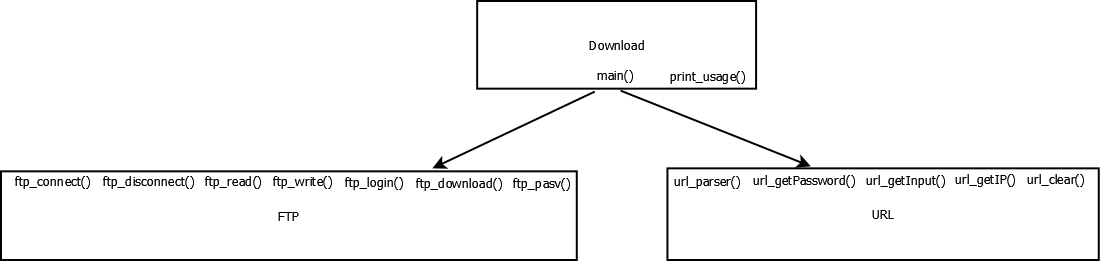
\includegraphics[width=0.95\textwidth]{Parte1.png}
    \caption{Arquitetura da aplicação download}
\end{figure}


A aplicação consiste em três componentes: FTP, URL e download.
O componente FTP é responsável pela comunicação com o servidor FTP usando Berkeley Sockets. As suas funções fornecem os meios para o estabelecimento das conexões TCP (controlo e dados), a terminação dessas conexões, e a transferência de dados. Este componente não tem visibilidade para nenhum dos outros componentes da aplicação.
O componente URL é responsável por fazer parser do URL FTP passado para a aplicação como argumento na linha de comandos, retirando o host, path, user e password. Caso um, ou vários, destes parâmetros estejam em falta, URL também fornece os meios para os obter perguntando ao utilizador para os introduzir. Este componente também não tem visibilidade para nenhum dos outros componentes da aplicação.
O componente download utilza os outros componentes para fazer o download do ficheiro.

\subsubsection{Componente FTP}
O componete FTP estabelece a ligação FTP na função ftp\_connect(), utilizando Berkeley Sockets para estabelecer as conexões TCP. O file descriptor data\_socket\_fd corresponde à conexão de dados e control\_socket\_fd à conexão de controlo.

\subsubsection{Componente URL}
Cada um das strings da estrutura URL correspondem a parâmetros necessários no estabelecimento da conexão FTP e no download do ficheiro e são retirados do URL recebido como argumento da linha de comandos ou inserida pelo utilizador. Caso o utilizador não tenha especificado a password no argumento da linha de comandos, então é pedida sem haver echo, não sendo mostrada no monitor e sendo uma alternativa mais segura para a introdução da password.

\subsubsection{Successful Download}
Foi testado a aplicação de download usando vários servidores FTP da FEUP, incluindo ftp.up.pt, pinguim.fe.up.pt e mirrors.fe.up.pt. Todos os download foram efetuados com sucesso, incluindo os testados na experiência 6 e na demostração da aplicação.

\section{Parte 2}

\subsection{Experiência 1}

\begin{figure}[h]
    \centering
    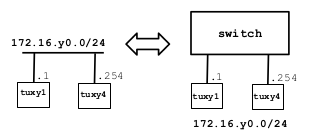
\includegraphics[width=0.50\textwidth]{ArquitecturaNasExperiencias/exp1.png}
    \caption{Arquitetura da experiência 1}
\end{figure}

\subsubsection{Objetivos}
Tentar interligar dois computadores através de um switch. E entender o funcionamento do protocolo ARP e do comando ping.

\subsubsection{Comandos principais de configuração}
Foi dado reset aos equipamentos:
\begin{verbatim}
Computadores,
    updateimage
Switch,
    no vlan 1-4094
    copy flash:tux5-clean startup-config
    reload
\end{verbatim}

E ligados os cabos do tux1(eth0) e tux4(eth0) ao switch. E configurados os ips de cada uma dessas interfaces:
\begin{verbatim}
Tux1,
    ifconfig eth0 172.16.50.1/24
Tux4,
    ifconfig eth0 172.16.50.254/24
\end{verbatim}

E apagadas cada uma das linhas da arp table para cada um dos pcs:
\begin{verbatim}
arp -d ipaddress
\end{verbatim}

\subsubsection{Análise das capturas}
Uma vez que foram apagadas as linhas da arp table torna-se crucial investigar
que máquina tem um dado ip. Tal é visível nos logs do wireshark, devido ao ping
que fizemos para o tux4(ping 172.16.50.254). Do tux1 é feito um broadcast de
uma trama do tipo ARP (Opcode) Request, que contém: o endereço IP do alvo; e a sua informação,
ip e mac. Ficando à espera da resposta do alvo. Quando o tux4 capta esta
mensagem, aceita-a porque tem o mesmo ip que o ip destino, e envia em unicast
uma trama do tipo ARP Reply contendo o seu endereço MAC, juntamento com todos os outros
dados.

\begin{figure}[h]
    \centering
    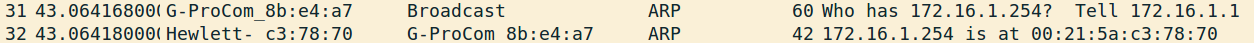
\includegraphics[width=0.95\textwidth]{exp1_arp.png}
    \caption{Trama EthernetII do tipo ARP}
\end{figure}
\begin{figure}[h]
    \centering
    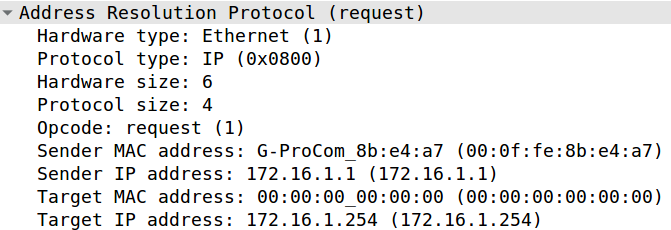
\includegraphics[width=0.60\textwidth]{exp1_arpBroadcast.png}
    \caption{Payload da trama EthernetII do tipo ARP, mais concretamente Request}
\end{figure}
\begin{figure}[h]
    \centering
    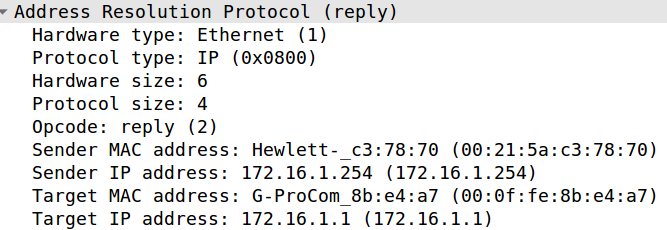
\includegraphics[width=0.60\textwidth]{exp1_arpReply.png}
    \caption{Payload da trama EthernetII do tipo ARP, mais concretamente Reply}
\end{figure}

Quando o tux1 recebe esta mensagem é inserida uma entrada na sua ARP table, com
o IP (network layer) e mac address (link layer) do tux4. O mesmo acontece ao
tux4 se tiver a ARP table sem uma linha para 172.16.50.1. Para além disto,
observámos que o comando ping gera um pacote Echo Request e espera por um Echo
Reply do host alvo, sendo que os endereços do network layer e da link layer
estão bem definidos e encontram-se respetivamente: na header do pacote, e no
header do EthernetII Frame(depende das máquinas pode onde a trama passa).
Verificou-se também que há um campo na header da EthernetII frame que indica o
tipo de protocolo, por exemplo se é ARP, IP ou ICMP. No entanto, não existe
nenhum campo em que seja especificado o tamanho da trama (ao contrário do que
acontece no pacote IP). Isto, deve-se ao facto do Physical Layer ter mecanismos
de reconhecimento do início e fim de uma trama, dependentes da codificação e do
meio de transmissão. Concluímos também que não é necessário haver um switch
para uma máquina falar com ela própria, uma vez que existe uma rede de
interfaces virtuais(loopback) que permitem isso mesmo. Necessário para: testar
configurações; correr servidores localmente; fazer simulações de redes; etc. De
modo rápido.

\subsection{Experiência 2}

\begin{figure}[h]
    \centering
    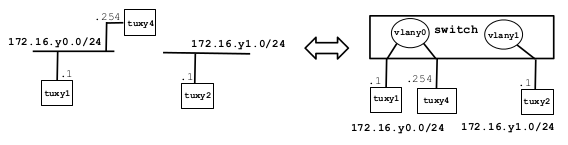
\includegraphics[width=0.70\textwidth]{ArquitecturaNasExperiencias/exp2.png}
    \caption{Arquitetura da experiência 2}
\end{figure}

\subsubsection{Objetivos}
Criação de duas LANs virtuais no switch, uma constituída pelo tuxy1 e tuxy4 e outro pelo tuxy2.
Visto que se encontram em sub-redes diferentes, tuxy1 e tuxy4 não conseguem comunicar com tuxy2.

\subsubsection{Comandos principais de configuração}
Para configurar o switch conectou-se a porta série de uma das máquinas com o switch e usou-se o programa gtkterm para inserir os comandos necessários.
Para adicionar cada uma das vlans ao switch, entrou-se na consola de configuração e criou-se a vlan com o identificador x0 usando os comandos:
\begin{verbatim}
configure terminal
vlan x0
end
show vlan id x0
\end{verbatim}
Cada máquina foi ligada a uma porta do switch, configurou-se uma Fast Ethernet Interface para cada porta, e ligou-se as portas cujas máquinas tuxy1 e tuxy4 se conectaram à vlany0 e a porta da máquina tuxy2 à vlany1, usandos os comandos:
\begin{verbatim}
configure terminal
interface fastEthernet 0/porta
switchport mode access
switchport access vlan x0
end
\end{verbatim}
Verificando as configurações:
\begin{verbatim}
show running-config interface fastEthernet 0/porta
show interfaces fastEthernet 0/porta switchport
\end{verbatim}

Por exemplo:
\begin{verbatim}
50	VLAN0050									active		Fa0/1, Fa0/2
51 	VLAN0051									active		Fa0/3
\end{verbatim}

De modo a não serem ignorados broadcasts de icmp echo:
\begin{verbatim}
echo 0 > /proc/sys/net/ipv4/icmp_echo_ignore_broadcasts
\end{verbatim}

\subsubsection{Análise das capturas}
Foi executando um ping da máquina tuxy1 para a máquina tuxy4 o que foi possível visto que se encontram na mesma vlan, e o ping entre tux1 e tuxy2 não foi executado com sucesso, pois pertencem a vlans diferentes.
Existem dois domínios de broadcast, devido a existir duas vlans (sem interligação entre elas).
Através dos logs verificamos que quando fazemos broadcast no tuxy1 só o tuxy4 responde. E quando
fazemos broadcast no tuxy2 nenhuma máquina responde, porque não chega nenhum pedido às
outras máquinas.

\subsection{Experiência 3}

\begin{figure}[h]
    \centering
    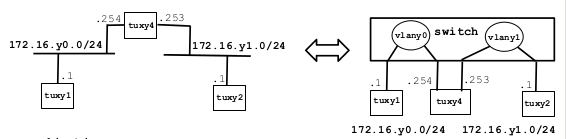
\includegraphics[width=0.50\textwidth]{ArquitecturaNasExperiencias/exp3.png}
    \caption{Arquitetura da experiência 3}
\end{figure}

\subsubsection{Objetivos}
Transformar a máquina tuxy4 num router, permitindo a comunicação entre as duas sub-redes criadas na experiência anterior.

Foi configurada a interface eth1 da máquina tuxy4 com IP 172.16.y1.253 e adicionada à vlan do tuxy2 (vlany1).

Para que possa haver routing da parte do tuxy4 e para haver comunicação entre as sub-redes ativou-se o IP fowarding no tuxy4(router):
\begin{verbatim}
	echo 1 > /proc/sys/net/ipv4/ip_foward
\end{verbatim}

No tuxy1 foi adicionada uma rota para a vlany1:
\begin{verbatim}
	route add –net 172.16.y1.0/24 gw 172.16.y0.254
	route -n
\end{verbatim}

\begin{tabular}{l l l l l l l l}
Destination & Gateway & Genmask & Flags & Metric & Ref & Use & Iface \\
172.16.50.0 & 0.0.0.0 & 255.255.255.0 & U & 0 & 0 & 0 & eth0 \\
172.16.51.0 & 172.16.50.254 & 255.255.255.0 & UG & 0 & 0 & 0 & eth0
\end{tabular} \\

Esta entrada na routing table faz com que haja um redirecionamento dos ips to tipo 172.16.y1.0/24 para o gateway router
172.16.y0.254(eth0 tuxy4). A primeira entrada da routing table tem o significado de aceitar o tráfego proveniente de 172.16.50.0/24.

Faz-se o mesmo para o tuxy2, adicionando uma rota para a vlany0:
\begin{verbatim}
	route add –net 172.16.y0.0/24 gw 172.16.y1.253
	route -n
\end{verbatim}

\begin{tabular}{l l l l l l l l}
Destination & Gateway & Genmask & Flags & Metric & Ref & Use & Iface \\
172.16.50.0 & 172.16.51.253 & 255.255.255.0 & UG & 0 & 0 & 0 & eth0 \\
172.16.51.0 & 0.0.0.0 & 255.255.255.0 & Ui & 0 & 0 & 0 & eth0
\end{tabular} \\

Faz forward dos ips 172.16.y0.0/24 para gateway router 172.16.y1.253(eth1 tuxy4). Aceita os ips provenientes da rede 172.16.51.0/24.

Tux4 funciona como um gateway router, pois redireciona de uma interface (eth0) para outra (eth1).

\begin{tabular}{l l l l l l l l}
Destination & Gateway & Genmask & Flags & Metric & Ref & Use & Iface \\
172.16.50.0 & 0.0.0.0 & 255.255.255.0 & U & 0 & 0 & 0 & eth0 \\
172.16.51.0 & 0.0.0.0 & 255.255.255.0 & U & 0 & 0 & 0 & eth1
\end{tabular} \\

Aceita o tráfego proveniente destas redes e não envia para nenhum gateway visto que os clientes
estão ligados diretamente, isto é, não há um decremento do ttl.

Para que os pacotes echos ICMP enviados em broadcasts não sejam automaticamente ignorados, é usado o seguinte comando:
\begin{verbatim}
	echo 0 > /proc/sys/net/ipv4/icmp_echo_ignore_broadcasts
\end{verbatim}

MAC addresses observadas:
\begin{verbatim}
HWaddr 00:21:5a:c3:78:70, é o mac address da interface eth0(172.16.50.254) do tux4.
HWaddr 00:c0:df:08:d5:b0, é o mac address da interface eth1(172.16.51.253) do tux4.
HWaddr 00:0f:fe:8b:e4:a7, é o mac address da interface eth0(172.16.50.1) do tux1.
HWaddr 00:21:5a:61:2f:d6, é o mac address da interface eth0(172.16.51.1) do tux2.
\end{verbatim}

\subsubsection{Análise das capturas}
Pode-se observar nos logs que naturalmente depois da configurações referidas é possível fazer ping do tuxy1 para todas as outras interfaces.
Após limpar as ARP tables das três máquinas fez-se ping do tuxy1 para o tuxy2, e é possível observar nos logs que uma vez que a ethernet usa MAC addresses e a ARP table foi limpa, o tuxy1 precisa de saber qual o mac address da interface eth0 do tuxy4, o tuxy4 precisa de saber o mac do tuxy2, o tuxy2 o mac do eth1 tuxy4, e o tuxy4 o mac do tuxy1. Tuxy1 envia um ARP request para obter o MAC address de eth0 tuxy4 e tuxy2 envia um ARP request a eth1 tuxy4.
É possível observar que os pacotes ICMP echo, request(tipo 8) e reply(tipo 0) presentes nos logs, são reencaminhados para o tuxy4. Estes são visíveis pelo tuxy4, em ambas as interfaces. Acontece uma coisa um pouco estranha que é o facto do tux3 parecer estar a fazer reply sem antes saber o mac do tux4 eth1 (através dos logs do wireshark). Só depois de algum tempo é que se vê o broadcast ARP a partir do tux3. Pensamos que isto é devido ao tux3 ter respondido ao broadcast do tux4, e de ter ficado de modo implícito com o mac do tux4 eth1 em cache, sendo só depois feito o pedido formal. O mesmo acontece do tux4 para o tux1.

\begin{figure}[h]
    \centering
    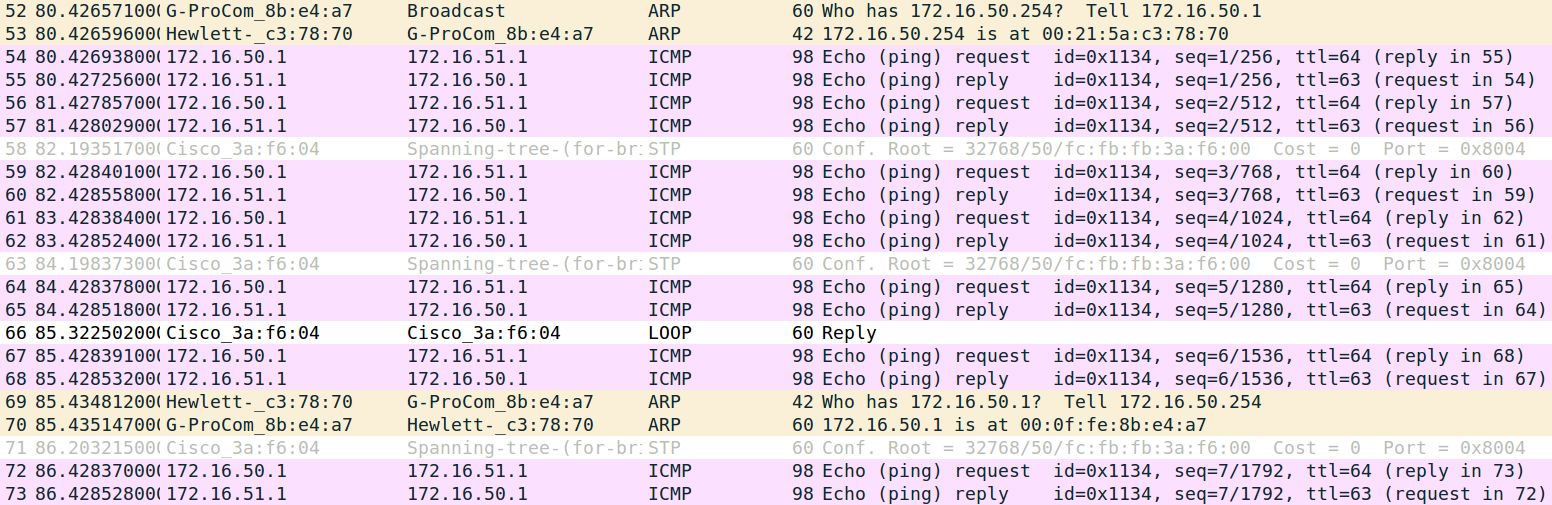
\includegraphics[width=0.95\textwidth]{exp3_logs.png}
    \caption{Comunicações na interface eth0 do Tux4}
\end{figure}

\subsection{Experiência 4}

\subsubsection{Objetivos}
Configurar um router comercial configurado com NAT de modo a termos accesso à
internet através da topologia da rede criada.

\subsubsection{Comandos principais de configuração}

Dar reset aos computadores e ao switch através dos comandos já apresentados.\\

Dar reset ao router através do seguinte comando:
\begin{verbatim}
    copy flash:tux5-clean startup-config
    reload
\end{verbatim}

Configurar cada pc com o ip correcto:
\begin{verbatim}
tux1,
    ifconfig eth0 172.16.50.1/24
tux2,
    ifconfig eth0 172.16.51.1/24
tux4,
    ifconfig eth0 172.16.50.254/24
    ifconfig eth1 172.16.51.253/24
\end{verbatim}

Configurar as routes para os pcs:
\begin{verbatim}
tux1,
    route add default gw 172.16.50.254
tux2,
    route add default gw 172.16.51.254
    route add -net 172.16.50.0/24 gw 172.16.51.253
tux4,
    route add default gw 172.16.51.254
\end{verbatim}

Criar as vlans como anteriormente demonstrado. E permitir o redirecionamento de pacotes no tux4:
\begin{verbatim}
echo 1 > /proc/sys/net/ipv4/ip_forward
\end{verbatim}

Configurar o router cisco com nat:
\begin{verbatim}
conf t
interface gigabitethernet 0/0
ip address 172.16.51.254 255.255.255.0
no shutdown
ip nat inside # Interface do lado lan
exit
interface gigabitethernet 0/1
ip address 172.16.1.59 255.255.255.0
no shutdown
ip nat outside # Interface do lado “wan”
exit
ip nat pool ovrld 172.16.1.59 172.16.1.59 prefix 24
ip nat inside source list 1 pool ovrld overload
# Esta permissão não deixa que o tux4 tenha acesso à net
# 0.0.0.255 para as permissões serem iguais para os hosts
access-list 1 permit 172.16.50.0 0.0.0.7
access-list 1 permit 172.16.51.0 0.0.0.7
# Default gateway do router com nat
ip route 0.0.0.0 0.0.0.0 172.16.1.254
# Para falar com os hosts do outro lado do router
ip route 172.16.50.0 255.255.255.0 172.16.51.253
end
\end{verbatim}

\subsubsection{Análise das capturas}
Na primeira captura do wireshark observamos que são descobertos os mac adresses
através do protocolo layer 2, ARP. Ao remover a route 172.16.y0.0/24 via tux4
do tux2, observámos que o pacote Echo Reply passa pelo router cisco, que por
sua vez redireciona para o router linux(tux4), chegando por fim ao tux1 por
forwarding do tux4. A introdução dessa route previne passar pelo router cisco,
aumentando assim a velocidade da conexão. Esta diferença deve-se ao algoritmo
das forwarding tables e das entradas presentes em cada máquina. Verificou-se
também que, quando o nat não está implementado é possível fazer pedidos para
fora da nossa rede, só que a resposta nunca chega.

\begin{figure}[h]
    \centering
    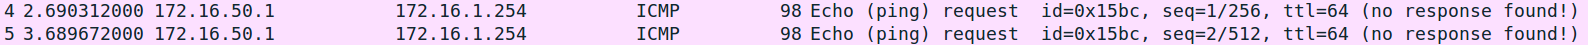
\includegraphics[width=0.95\textwidth]{exp4_whynat.png}
    \caption{Não há resposta sem NAT}
\end{figure}

Isto, deve-se ao facto do router cisco não saber para que host enviar uma dada
trama. Daí ser necessário a funcionalidade NAT. Como constatámos, esta técnica
permite utilizar os mesmos ips em diferentes redes, chamadas redes
privadas(10.0.0.0/8, 172.16.0.0/12, 192.168.0.0/16). Isto é possível porque os
ips privados são traduzidos para um público. Este mapeamento é feito através de
uma tabela chamada tabela de tradução de endereços de rede, que possibilita que
o router saiba para que hosts são destinados certos pacotes vindos da internet.
Cada entrada da tabela tem uma parte para o lado WAN e outra para o lado LAN,
cada um deles tem dois campos: um para o ip e a outra para a porta. A porta é o
que permite fazer a distinção entre destinos de pacotes. É possível
reencaminhar todos os pacotes wan com destino a uma dada porta (por exemplo,
porta default para o server http, 80) para uma dada porta de um host, que terá
um processo em modo listening associado a essa porta.

\begin{figure}[h]
    \centering
    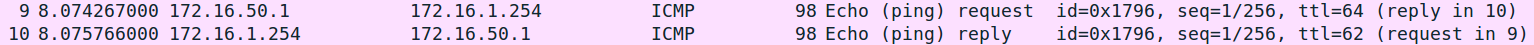
\includegraphics[width=0.95\textwidth]{exp4_nat.png}
    \caption{Há resposta visto NAT estar configurado}
\end{figure}

\subsection{Experiência 5}

\subsubsection{Objetivos}
Configurar o DNS de modo a conseguir acessar a redes externas, acedendo à Internet através da rede previamente criada.

A arquitetura da rede continuou igual à da experiência anterior.

Para configurar o serviço DNS alterou-se o ficheiro /etc/resolv.conf, em cada uma das máquinas. Nesta experiência o conteúdo deste ficheiro foi alterado para:

\begin{verbatim}
	search lixa.netlab.fe.up.pt
	nameserver 172.16.1.1
\end{verbatim}

172.16.1.1, é o endereço do servidor de nomes para onde se fazem os pedidos. lixa.netlab.fe.up.pt, é o único elemento da lista de procura de hostnames.

Existem três tipos de pacotes DNS: Queries, Responses e Updates. Os pacotes query e reponses(replies) têm um formato comum, para além dos 12 bytes do cabeçalho: identificação; flags; número de perguntas; número de respostas de RRs; número de registos de servidores authoritative; e, número adicional de RRs. São enviadas: perguntas com os campos nome e tipo(A, NS, CNAME e MX) selecionados; respostas a uma pergunta, RRs completos; registo de servidores authoritative; e, informação adicional útil. O pacote de update contém à semelhança dos outros um header com: uma identificação; flags; e, número de registo de recursos(RRs) para cada tipo da secção seguinte: zone entry; prerequisite resource records; update resource records; e, additional resource records.

\subsubsection{Análise das capturas}

É possível verificar a troca de pacotes DNS no início da ligação à Internet:
\begin{figure}[h]
    \centering
    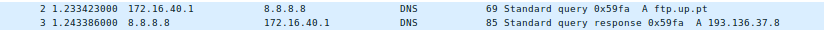
\includegraphics[width=0.95\textwidth]{exp5_dns.png}
    \caption{Pacotes DNS - Query e Response}
\end{figure}

Query:
\begin{verbatim}
	ftp.up.pt: type A, class IN
\end{verbatim}
Response:
\begin{verbatim}
	ftp.up.pt: type A, class IN, addr 193.136.37.8, Time to live: 3616, Data length: 4
\end{verbatim}

\subsection{Experiência 6}

\subsubsection{How many TCP connections are opened by your ftp application?}

São abertas duas conexões TCP pela aplicação FTP, uma de controlo e outra de dados.
Primeiramente a aplicação cria uma conexão TCP de controlo que conecta um porto sem privilégios (porto > 1023) ao porto FTP do servidor (porto 21) que vai continuar aberta durante a transferência.
Foi utilizado nesta aplicação o modo passivo por oposição ao modo activo, sendo o cliente a abrir a conexão TCP de dados.
No modo activo o cliente envia para o servidor um número de porto aleatório e sem privilégios, para se conectar e é o próprio servidor a abrir a conexão TCP de dados, ligando a porto do cliente recebido e o seu porto 20.
No modo passivo o servidor envia para o cliente um número de porto aleatório e sem privilégios, e é o cliente que abre a conexão TCP de dados.

\subsubsection{In what connection is transported the FTP control information?}

A informação de controlo FTP é transportada na conexão de controlo que liga um porto aleatótio do cliente e o porto 21 do servidor. É também transportado as mensagens de acknowledgement (ACK).

\subsubsection{What are the phases of a TCP connection?}

As três fases duma conexão TCP são: connection estabelishment, data transfer e connection termination.

\subsubsection{How does the ARQ TCP mechanism work? What are the relevant TCP
fields? What relevant information can be observed in the logs?}

O receptor não faz request de retransmissão de pacotes perdidos. O transmissor espera pelo ACK e quando
não o recebe, reenvia os pacotes após um certo intervalo. Pode ser implementado de várias formas (Stop-and-wait, Go-Back-N,
Selective Repeat).
O TCP header contém campos como o porto da fonte e o porto do destinatário, o número de sequência, o número de acknowledgement e
o tamanho da window.
É atribuido um número de sequência a cada byte de dados, sendo que o número de sequência do TCP header é o do primeiro byte de dados desse pacote. O número de acknowledge indica o número de sequência que o receptor espera do emissor e o tamanho da window indica o número de bytes que o receptor está disposto a receber.

\subsubsection{How does the TCP congestion control mechanism work? What are the
relevant fields. How did the throughput of the data connection evolve
along the time? Is it according to the TCP congestion control mechanism?}
Existem vários mecanismos de controlo de congestionamento TCP. Cada um deles possui algoritmos de controlo de congestionamento juntamento com outras abordagens. Por exemplo: Slow start; Congestion avoidance; Fast retransmit; Fast Recovery; etc. Exemplos de mecanismos que usam alguns destes algoritmos: TCP Tahoe; TCP Newreno; TCP Vegas; etc. Slow start, funciona através de acknowledgements e duas janelas, uma no receptor e outra no emissor estando o emissor dependente destas. Congestion avoidance, um timer de retransmissão, recepção de duplicados e a alerta desta situação ao emissor. Fast retransmit, maneira estratégica de lidar com ACKs duplicados de maneira a não haver esperas. O throughput evolui até um determinado ponto e diminui quando há congestionamento e depois retoma. Consequência do mecanismo exibir um cariz Slow start. O mecanismo pode ser observado em /proc/sys/net/ipv4/tcp\_congestion\_control.

\subsubsection{Is the throughput of a TCP data connections disturbed by the appearance of a second TCP connection? How?}
Sim existe conflitos devido à existência de outra conexão TCP. Isto pode ser verificado através das linhas pretas no wireshark que indicam erros de ZeroWindow, ACKed unseen segment, Fast Retransmission, TCP Previous segment not captured, etc.

\section{Conclusões}
%síntese da informação apresentada nas secções anteriores; reflexão sobre os
%objectivos de aprendizagem alcançados
A elaboração deste trabalho contribuiu para a aprendizagem dos conhecimentos
básicos do protocolo ftp, tal como o modo de estruturação e configuração de
componentes de uma rede de computadores. O projecto  desenvolvido resultou numa
aplicação capaz de fazer o download de ficheiros via ftp em modo passivo, com
ou sem autenticação. E numa rede atual funcional. O trabalho foi realizado com
sucesso e com grande entusiasmo, visto que, compreendemos a maneira como o
protocolo ftp funciona, como implementá-lo, e como criar a nossa própria rede de
computadores. A partir dos logs guardados durante as experiências podemos inspecionar
os pacotes transferidos, e adquirir um conhecimento mais aprofundado e mais prático dos protocolos,
FTP, TCP, ICMP, e LOOP. Este trabalho permitiu consolidar a matéria dada durante o semestre na cadeira
de Redes de Computadores. Goodbye MEO router, welcome openwrt :).

\end{document}
